\documentclass[a4paper]{article}

\usepackage[english]{babel}
\usepackage[utf8]{inputenc}
\usepackage{graphicx}
\usepackage[colorinlistoftodos]{todonotes}
\usepackage{listings}
\usepackage{xcolor}

\lstset{
    frame=tb,
    tabsize=4,
    showstringspaces=false,
    numbers=left,
    commentstyle=\color{green},
    keywordstyle=\color{blue},
    stringstyle=\color{red}
}

\title{Controllable Terrain}

\author{Edward Seim}

\date{Novemeber 12, 2014}

\begin{document}

\maketitle

\section{Summary}

The big problem for me with this assignment is the overview, do I move the whole actor or move the component within the actor. Real world use would determine this, but in general if its just a shift in terrain as opposed to full adjustment, I determined that would be a component movement. Looking into how to move a component within an actor, you are esentially moveing a component relative to the root, nowhere mentioning the world position its in, which makes sense when you think about it. Unreal made this component move even easier by not needing to create a timeline. In the case of moving the whole actor, I've had to create a timeline for the location the actor would be at each time as a graph of some sort. The compenent move simply asked for the final location relative to the root and what amount of time I wanted the animation to take. It even has booleans for acceleration at the beginning and/or end.

\section{Code Snapshot}

\begin{figure}
\centering
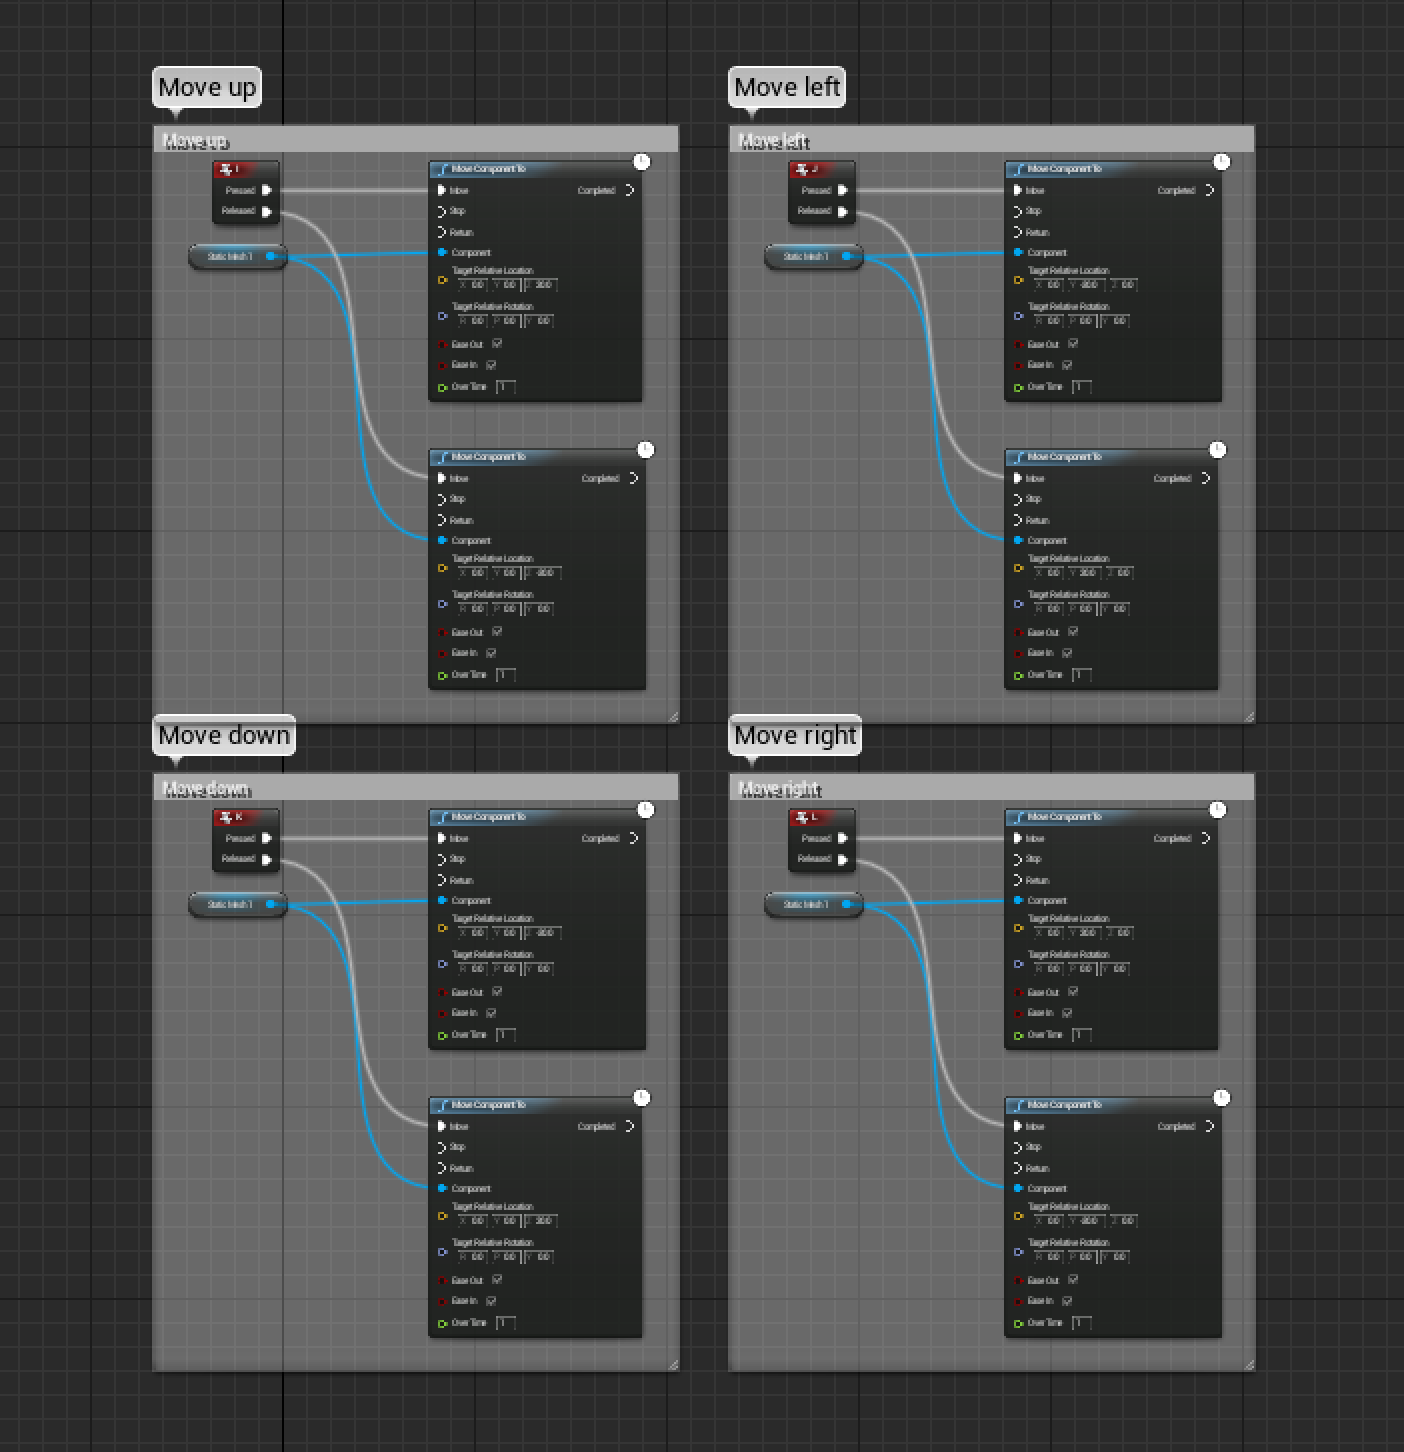
\includegraphics[keepaspectratio=true, scale=.4]{BlueprintOverview.png}
\includegraphics[keepaspectratio=true, scale=.4]{BlueprintExmpleSection.png}
\end{figure}

\end{document}